% patterns.meta Lines family only.
\usetikzlibrary{patterns.meta}

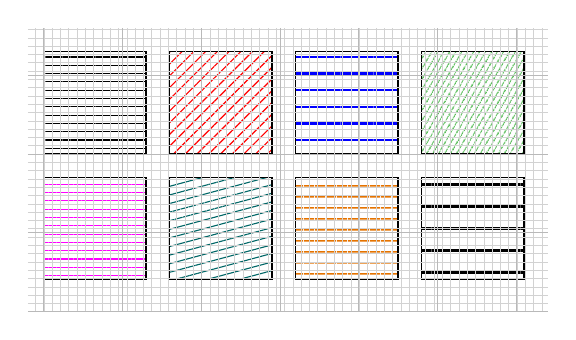
\begin{tikzpicture}[x=1cm,y=1cm]
  \path[draw,pattern={Lines},pattern color=black] (0,0) rectangle +(1.3,1.3);
  \path[draw,pattern={Lines[angle=45]},pattern color=red] (1.6,0) rectangle +(1.3,1.3);
  \path[draw,pattern={Lines[distance=6pt,line width=.8pt]},pattern color=blue] (3.2,0) rectangle +(1.3,1.3);
  \path[draw,pattern={Lines[distance={3pt/sqrt(2)},angle=60]},pattern color=green!60!black] (4.8,0) rectangle +(1.3,1.3);

  \path[draw,pattern={Lines[xshift=1pt,yshift=2pt]},pattern color=magenta] (0,-1.6) rectangle +(1.3,1.3);
  \path[draw,pattern={Lines[angle=15,xshift=2pt,yshift=-1pt]},pattern color=teal!80!black] (1.6,-1.6) rectangle +(1.3,1.3);
  \path[draw,pattern={Lines[distance=4pt,line width=.5pt]},pattern color=orange!90!black] (3.2,-1.6) rectangle +(1.3,1.3);
  \path[draw,pattern={Lines[distance=8pt,line width=1pt]},pattern color=black] (4.8,-1.6) rectangle +(1.3,1.3);

  % Overlay reference grid for easier phase/offset comparison.
  \draw[step=3pt,gray!35,line width=.1pt] (-0.2,-2.0) grid (6.4,1.6);
  \draw[step=1cm,gray!55,line width=.16pt] (-0.2,-2.0) grid (6.4,1.6);
\end{tikzpicture}
